%% Chapter3_Methodology.tex
\chapter{Research Methodology}
\label{chap:meth}

\section{Research Approach}
The work is simulation-based and experimental. A software-only approach was chosen because experiments on a real junction are costly, unsafe and not repeatable, whereas a simulator lets every controller see exactly the same arrivals. A seed fixes the random arrival sequence, so runs of different controllers form matched pairs; results are reported as means with 95\% confidence intervals and compared with paired $t$-tests. The system is built incrementally, milestone by milestone, and each milestone is fully working before the next begins. Control uses exact simulated vehicle states; the vision pipeline is evaluated alongside against exact ground truth, and a separate sensing experiment measures what imperfect sensing would cost.

\section{Proposed System / Algorithm / Framework}

\subsection{Overall Architecture and Workflow}
The system consists of Python packages with one-directional dependencies: the simulation core imports no decision, analytics or web code, and every signal controller implements one interface (an update per time step and a phase name), so fixed-time, adaptive and comparison controllers can be exchanged without changes elsewhere. Figure~\ref{fig:architecture} shows the architecture and Figure~\ref{fig:workflow} the method workflow: in every step the controller senses vehicle positions, speeds and classes, scores each approach, and decides whether the current green may end; the preemption layer then protects every transition with full yellow and all-red intervals before the signal heads change.

\begin{figure}[H]
\centering
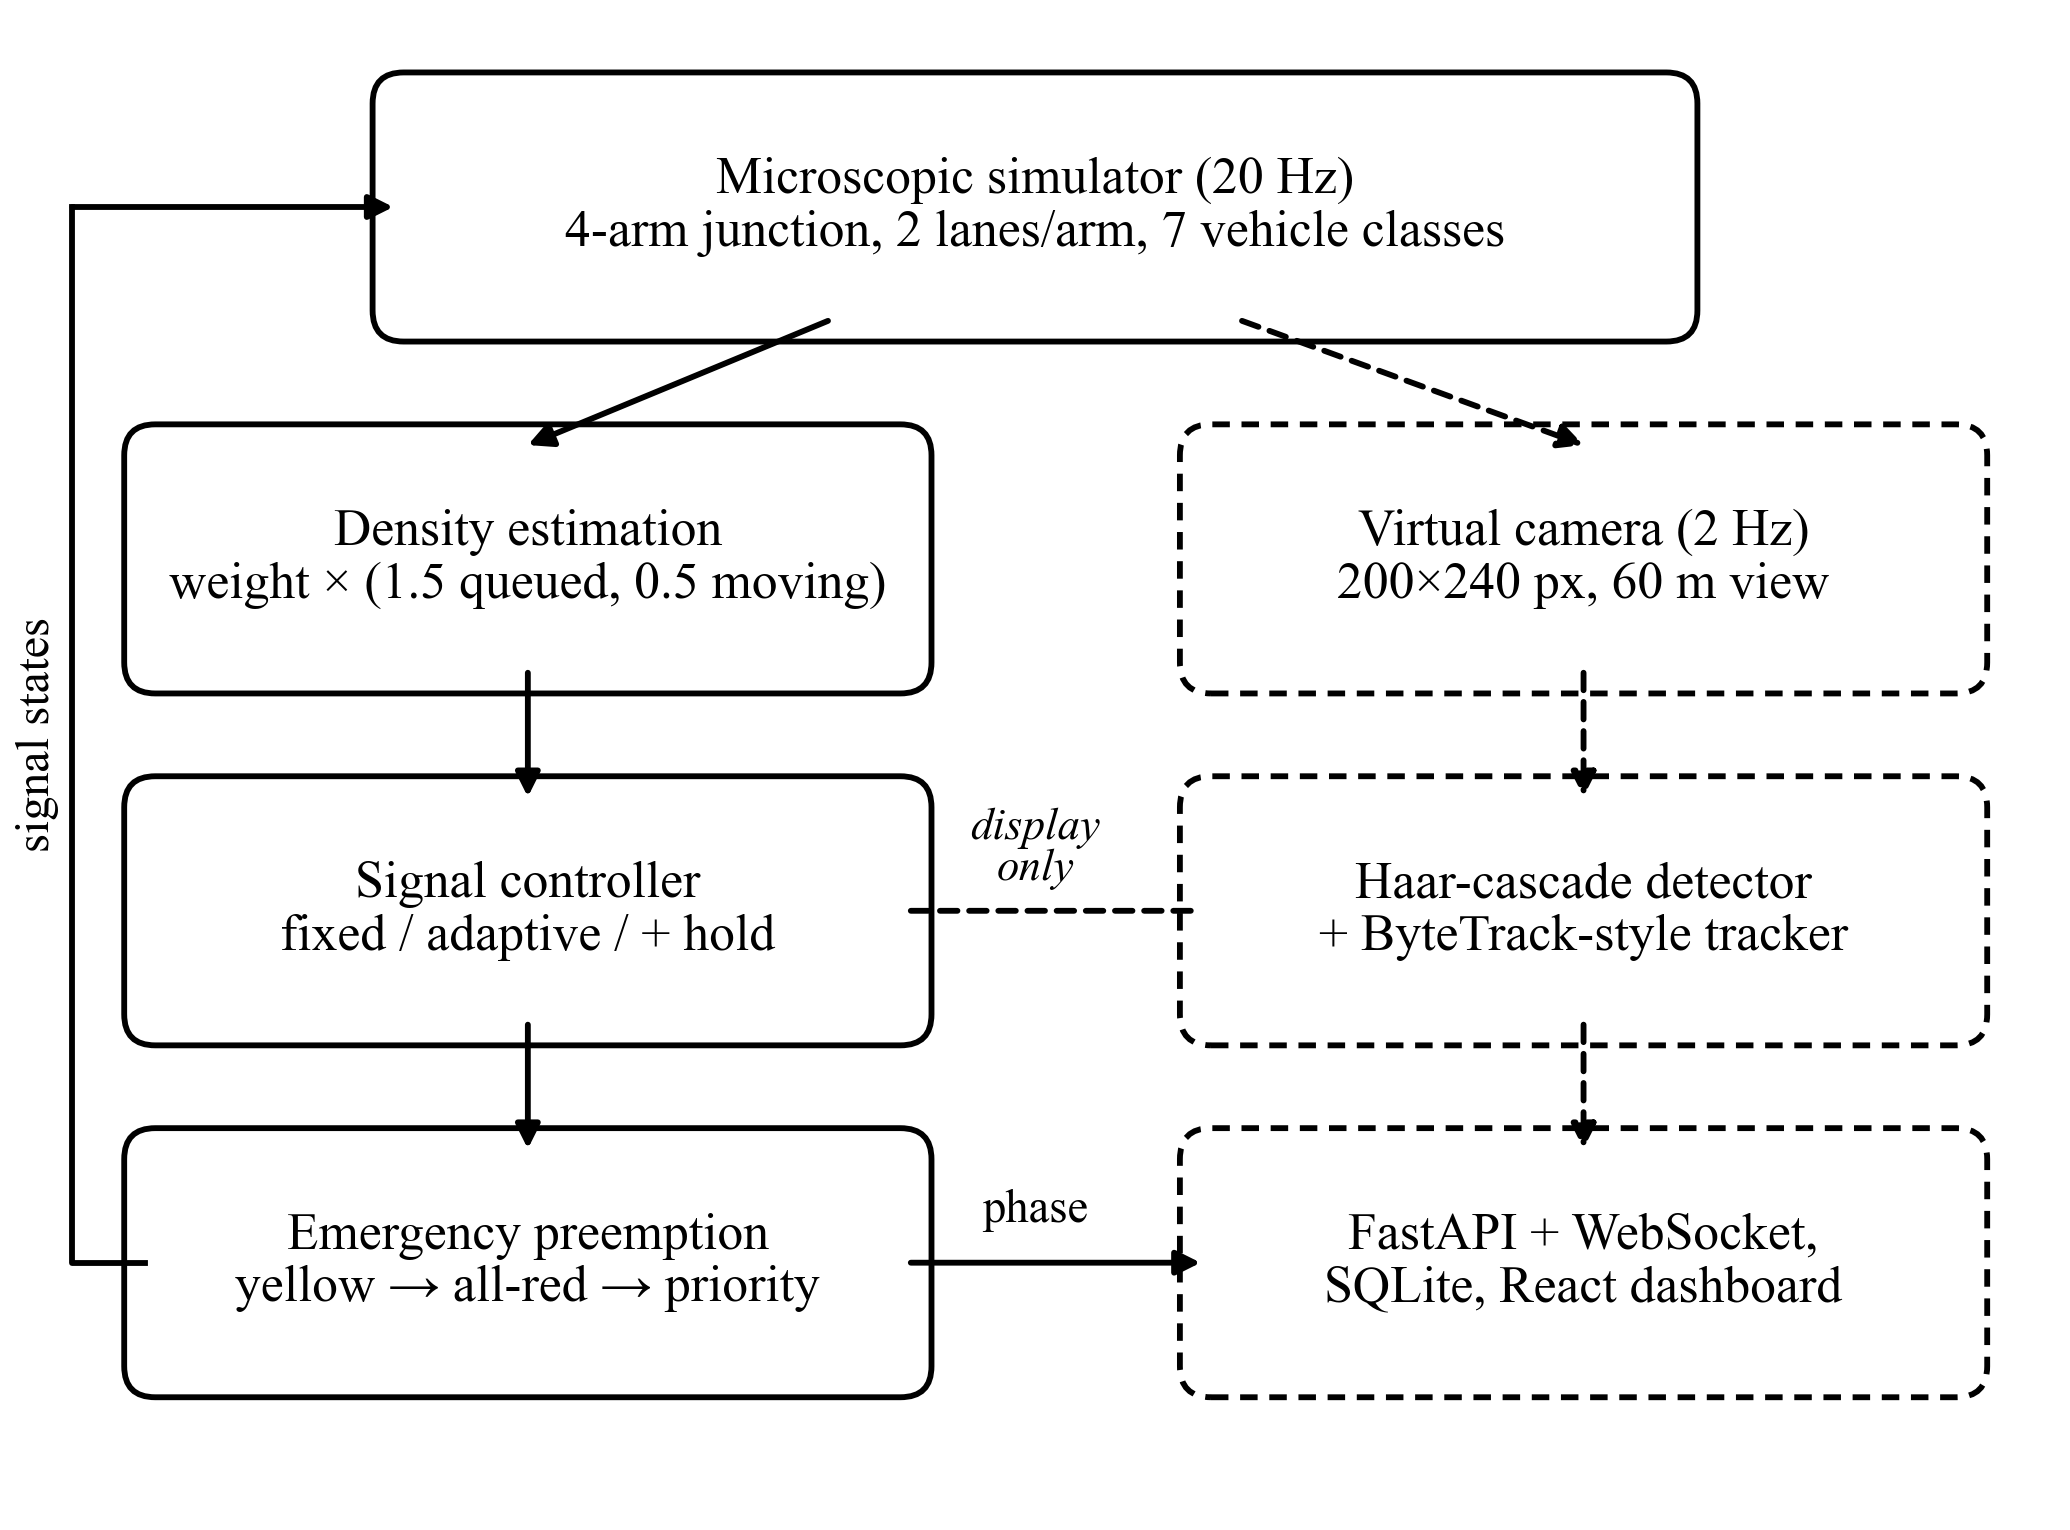
\includegraphics[width=0.75\textwidth]{figures/fig1_architecture.png}
\caption{Software architecture. Solid boxes form the control loop; dashed boxes form the vision pipeline, whose output is displayed and evaluated but not used for control in this study.}
\label{fig:architecture}
\end{figure}

\begin{figure}[H]
\centering
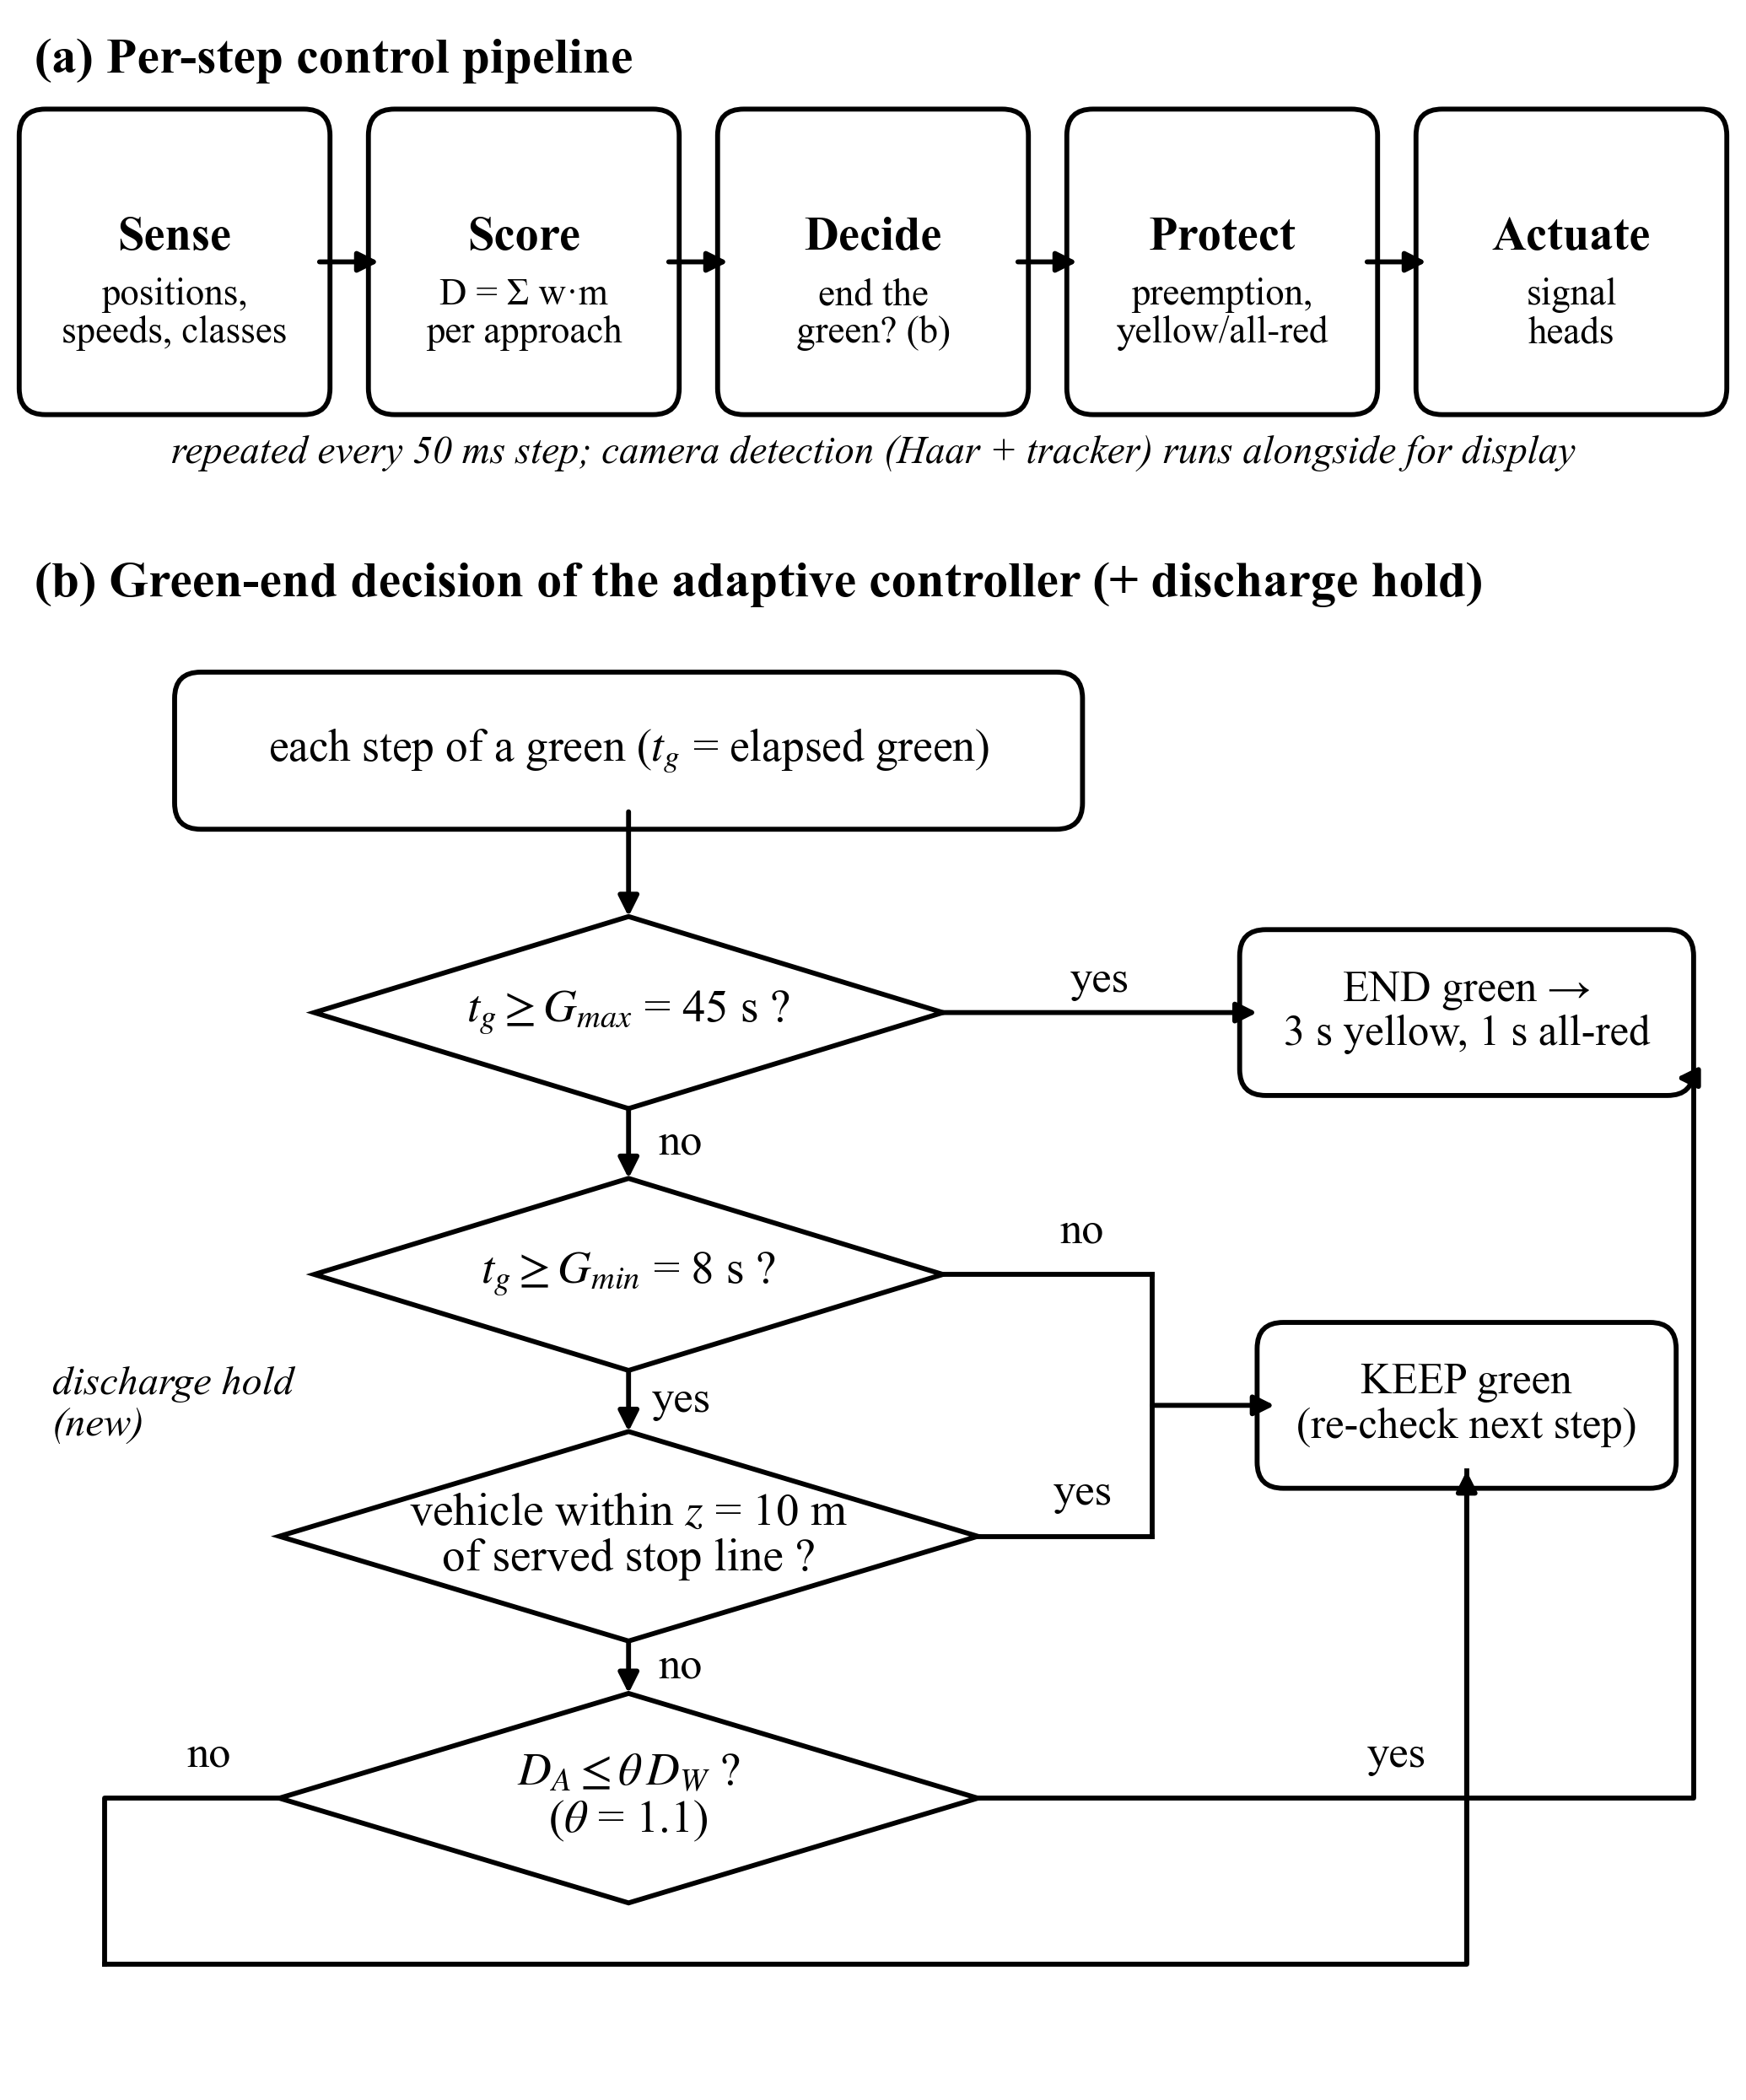
\includegraphics[width=0.62\textwidth]{figures/fig2_workflow.png}
\caption{Method workflow. (a) The per-step control pipeline. (b) The green-end decision; the test marked ``discharge hold'' is the extension added to the original controller.}
\label{fig:workflow}
\end{figure}


\subsection{Junction and Traffic Model}
The junction has four approaches, each with two lanes on a 330~m link; the stop line is at 200~m and the far edge of the junction box at 218~m. Vehicles travel straight through; turning movements, lane changes and pedestrians are not modelled. Vehicles arrive on each approach at a mean rate $\lambda$ with deterministic headways (one vehicle every $1/\lambda$~s); to create shifting imbalance, every 15~s the rate of each approach is redrawn as $\lambda\cdot U(0.4,1.6)$, with a floor of 0.02~veh/s. An arriving vehicle enters a lane at rest and is dropped if the rear of the previous vehicle is still within 8~m. For the above-capacity experiments two options are enabled instead: a blocked arrival waits in an entry queue and enters as soon as there is room, so that unserved demand and its waiting time are measured, and a vehicle enters at the highest speed from which it can still stop behind its leader. Table~\ref{tab:vehicles} lists the seven vehicle classes.

\begin{table}[H]
\centering
\caption{Vehicle classes and parameters used in the simulation}
\label{tab:vehicles}
\small
\resizebox{\ifdim\width>\textwidth\textwidth\else\width\fi}{!}{%
\begin{tabular}{lcccccc}
\toprule
\textbf{Class} & \textbf{Share (\%)} & \textbf{Length (m)} & \textbf{$v_{max}$ (m/s)} & \textbf{$a$ (m/s$^2$)} & \textbf{$b$ (m/s$^2$)} & \textbf{Weight $w$} \\
\midrule
Car & 55 & 4.5 & 14 & 2.5 & 4.5 & 1.0 \\
Motorcycle & 25 & 2.0 & 15 & 3.5 & 5.0 & 0.5 \\
Auto-rickshaw & 10 & 3.2 & 11 & 2.0 & 4.0 & 0.8 \\
Bus & 5 & 10.0 & 10 & 1.2 & 3.0 & 3.0 \\
Truck & 4 & 9.0 & 9 & 1.0 & 2.8 & 2.5 \\
Ambulance & 0.5 & 5.5 & 16 & 3.0 & 5.0 & 6.0 \\
Fire truck & 0.5 & 10.5 & 12 & 1.5 & 3.5 & 6.0 \\
\bottomrule
\end{tabular}}
\par\smallskip{\footnotesize $a$: maximum acceleration; $b$: maximum deceleration; $w$: density weight used in Eq.~\eqref{eq:density}.}
\end{table}


Longitudinal motion follows a Gipps-type safe-speed rule~\cite{ref21}. A follower's speed is limited to
\begin{equation}
u_{safe} = \sqrt{2b\left(g + \frac{u_l^{2}}{2b_l} - s_0\right)}
\label{eq:safe}
\end{equation}
where $g$ is the gap to the leader's rear, $u_l$ and $b_l$ are the leader's speed and maximum deceleration, $b$ is the follower's maximum deceleration and $s_0 = 2$~m is the standstill gap. A position constraint prevents any overlap within a step. On yellow or red, a vehicle upstream of the stop line brakes once its braking distance reaches the distance to the line; a vehicle too close to stop continues. Rule~\eqref{eq:safe} has no driver reaction time; Section~\ref{sec:kin} shows that this makes queues discharge too fast, adds a reaction time $\tau$, and repeats the main comparisons with it.

\subsection{Density Estimation}
For approach $r$ with vehicle set $V_r$, the density score is
\begin{equation}
D_r = \sum_{v\in V_r} w_{c(v)}\, m(v)
\label{eq:density}
\end{equation}
where $w_{c(v)}$ is the class weight (Table~\ref{tab:vehicles}) and $m(v) = 1.5$ if vehicle $v$ is queued and $0.5$ otherwise. A vehicle is queued when it is upstream of the stop line and slower than 0.5~m/s. The weights reflect the road space and discharge time a vehicle class needs, and emergency vehicles receive a high weight so that their approach is favoured even without preemption. A queued vehicle counts three times as much as a moving one because it needs green now, whereas a moving vehicle may still be far upstream. The weights are heuristic; Section~\ref{sec:ablation} measures the contribution of each part of the score and Section~\ref{sec:calib} calibrates them. For display, an approach is labelled low ($D_r \le 3$), medium ($3 < D_r \le 6$) or high ($D_r > 6$).

\subsection{Adaptive Green Extension}
The controller uses a two-phase plan: north--south green, yellow ($Y = 3$~s), all-red ($A = 1$~s), then east--west green, yellow and all-red. Only the green duration adapts. Let $t_g$ be the elapsed green time, and $D_A$ and $D_W$ the summed scores of the active and the waiting direction. At every step the green ends when
\begin{equation}
t_g \ge G_{max} \quad\text{or}\quad \bigl(t_g \ge G_{min} \;\text{and}\; D_A \le \theta D_W\bigr)
\label{eq:green}
\end{equation}
with $G_{min} = 8$~s, $G_{max} = 45$~s and $\theta = 1.1$. The green is thus extended while the served direction's score exceeds the waiting direction's by more than 10\%. Because yellow and all-red are fixed and green is capped, the red time of any approach in normal operation is bounded by
\begin{equation}
R_{max} = A + G_{max} + Y + A = 50\ \text{s}
\label{eq:rmax}
\end{equation}
so no approach can be starved. The fixed-time baseline uses the same sequence with a 20~s green (48~s cycle).

\subsection{Discharge Hold}
\label{sec:hold}
Rule~\eqref{eq:green} has a weakness that the above-capacity experiments expose (Section~\ref{sec:cap}). When both directions are saturated, the vehicles moving off on green score 0.5 each while the queue growing on red scores 1.5 each, so $D_A \le \theta D_W$ holds soon after $G_{min}$ and greens stay short; each phase change costs $Y + A = 4$~s in which no vehicle is served, so short greens lose capacity exactly when it is scarcest. The discharge hold adds the gap-out test of actuated control~\cite{ref23}: past the minimum, a green may only end once the served direction has gapped out, i.e.\ no served vehicle is within $z$ of its stop line,
\begin{equation}
t_g \ge G_{max} \quad\text{or}\quad \bigl(t_g \ge G_{min} \;\text{and}\; n_z = 0 \;\text{and}\; D_A \le \theta D_W\bigr)
\label{eq:hold}
\end{equation}
where $n_z$ is the number of served vehicles within $z = 10$~m upstream of the stop line. A saturated queue moving off always keeps a vehicle at the line and so keeps its green up to $G_{max}$, while free-flowing arrivals cross 10~m in under a second, so a cleared queue still hands over early. The zone length was chosen from 10, 15, 20 and 30~m on a separate tuning seed that is not used in any reported result. Yellow, all-red and the green limits are unchanged, so bound~\eqref{eq:rmax} still holds.

\subsection{Comparison Controllers}
To compare against existing approaches (Chapter~\ref{chap:lit}), four strategies were re-implemented in the same simulator. They are not the original systems: like the proposed controller they read exact vehicle states, and all share its phase sequence, its 3~s yellow and 1~s all-red, and its 8--45~s green limits, so every one obeys bound~\eqref{eq:rmax} and the comparison isolates the switching decision.
\begin{itemize}
  \item \textbf{Webster fixed:} a fixed plan whose green follows Webster's formula~\cite{ref2} for the mean demand of each run: $C_0 = (1.5L + 5)/(1 - Y_f)$, with lost time $L = 8$~s, $Y_f$ the sum of the critical flow ratios $q/s$, the saturation flow $s = 6000$~veh/h per approach measured in the simulator, and each phase receiving $(C_0 - L)/2$, clamped to 8--45~s. It knows the true mean demand of the run, which favours it.
  \item \textbf{Actuated:} past the minimum, the green ends as soon as the served direction gaps out (no vehicle within 10~m of its stop line) and a vehicle waits on the other direction~\cite{ref23}; no density score is used.
  \item \textbf{Max-pressure:} the pressure of a phase is the number of vehicles upstream of its stop lines minus those downstream, which is zero with free exits~\cite{ref11}; past the minimum the controller switches as soon as the waiting phase's pressure exceeds the served one's. This also represents busiest-lane-first control~\cite{ref6}.
  \item \textbf{Density levels:} following~\cite{ref1}, when a green starts the served direction's density is classed low, medium or high and the green is set to 10, 20 or 30~s, without revision during the green.
\end{itemize}

\subsection{Emergency Vehicle Preemption}
Preemption is a wrapper around any phase-based controller (Figure~\ref{fig:preemption}). Without an emergency vehicle it passes control to the inner controller. When an ambulance or fire truck is upstream of the junction exit, it acts as follows.
\begin{itemize}
  \item \textbf{Entry:} a conflicting green first shows a full 3~s yellow, and a yellow already showing keeps its remaining time; all approaches are then red for 1~s, or for the remainder of an all-red already under way. If the emergency vehicle's approach is already green, that green is held.
  \item \textbf{Priority green:} the emergency vehicle's direction (both opposing approaches) is green until no emergency vehicle remains before the junction exit, or for at most 20~s.
  \item \textbf{Release:} the priority green ends with a full yellow and all-red, after which the inner controller restarts at the green of the direction that was held.
  \item \textbf{Minimum green:} a green shown for less than 5~s is never cut, and an approach that already has green is served first.
\end{itemize}
When no other preemption is active, an emergency vehicle waits at most $5 + 3 + 1 = 9$~s for its priority green. Emergency vehicles are detected from the simulator state, i.e.\ perfect detection is assumed; in practice the input could come from vehicle-to-infrastructure messages or visual sensing.

\begin{figure}[H]
\centering
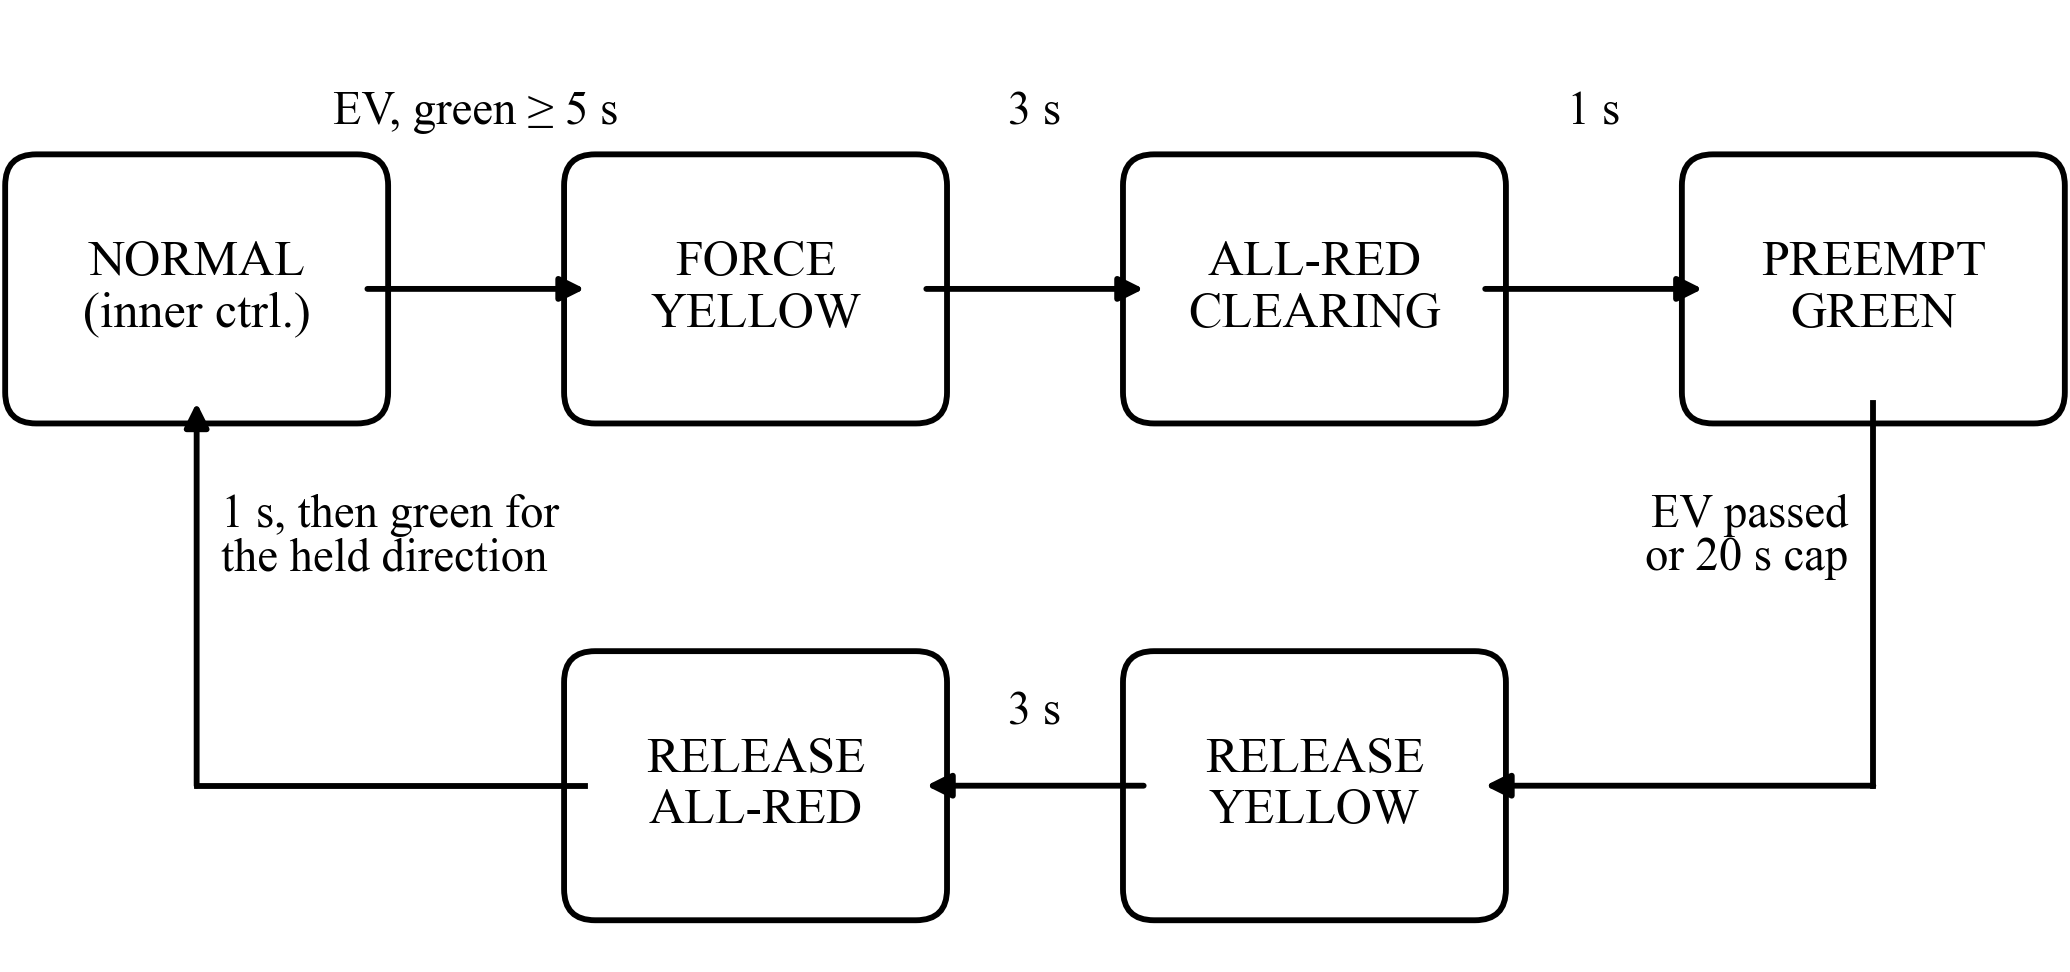
\includegraphics[width=0.85\textwidth]{figures/fig3_preemption.png}
\caption{Emergency preemption states. Every path from one direction's green to the other's passes through a full yellow and all-red interval.}
\label{fig:preemption}
\end{figure}


\subsection{Vision Pipeline}
For each approach a virtual camera renders a $200\times240$ pixel frame of the 60~m before the stop line (4~px/m). Vehicles appear as shaded rectangles with a windshield band on a noisy road texture with lane markings. The detector converts the frame to grayscale, equalizes its histogram, upscales it three times, and applies OpenCV's cascade classifier with a pre-trained vehicle cascade~\cite{ref16} (scale factor 1.05, minimum neighbours 2, minimum size 20~px); the final-stage weight, clipped to $[0,1]$, serves as a relative confidence. A single cascade localizes vehicles but does not classify them, so on its own it cannot supply the class weights of Eq.~\eqref{eq:density}.

The tracker keeps a constant-velocity Kalman filter~\cite{ref18} on each box centre and matches predicted boxes to detections with the Hungarian algorithm~\cite{ref19} on an IoU cost (minimum IoU 0.15). As in ByteTrack~\cite{ref17}, detections with confidence $\ge 0.15$ are matched first and the remaining low-confidence detections are then matched to still-unmatched tracks; only confident detections start tracks. A track is confirmed after two matches and deleted after three frames without one.

\section{Tools, Technologies, and Platforms}

\begin{table}[H]
\centering
\caption{Tools and Technologies Used}
\label{tab:tools}
\small
\begin{tabular}{@{}p{3.5cm}p{5cm}p{6cm}@{}}
\toprule
\textbf{Category} & \textbf{Tool / Technology} & \textbf{Purpose} \\
\midrule
Programming Language & Python 3.12; JavaScript (ES modules) & Simulation, decision engine, backend; dashboard \\
Numerical / Vision   & NumPy 2.1, SciPy 1.14, OpenCV 4.10 (headless) & Statistics and Hungarian assignment; Haar cascade and image processing \\
Backend Framework    & FastAPI 0.115, Uvicorn, Pydantic 2.9, WebSockets 13 & REST API and live streaming \\
Frontend Framework   & React 18, Vite 5, Tailwind CSS 3, Recharts 2 & Live dashboard and analytics charts \\
Database             & SQLite via SQLAlchemy 2.0 and aiosqlite (PostgreSQL-ready) & Snapshots, events, report export \\
Testing / CI         & pytest 8, httpx; GitHub Actions & 119 automated tests; build and Docker smoke test \\
Packaging            & Docker and Docker Compose & Two-container deployment \\
Hardware (optional)  & Raspberry Pi (GPIO) / ESP32 & Mirror the controller's signal on LEDs or relays \\
Version Control      & Git + GitHub & Collaboration and backup \\
IDE                  & VS Code & Development \\
\bottomrule
\end{tabular}
\end{table}

\section{Data Collection and Analysis}
No real images or field data are used. Traffic is generated by the simulator with seeded random arrivals, and the camera frames and their ground-truth boxes are both rendered from the same simulator state, so annotation is automatic, exact and involves no manual labelling. Nothing is trained: the cascade is pre-trained, the controller is rule-based, and the detector and tracker parameters were fixed during development in unseeded runs, so there is no training split. Three kinds of seeds are kept apart: seed 1000 for tuning (the hold zone), seeds 101--105 for capacity measurement, and seeds 1--10 for all reported results (seeds 1--4 for the vision evaluation). In total 3,524 simulation runs (1,797.0 simulated hours) were made.

Three demand levels below capacity were simulated: $\lambda = 0.08$, $0.12$ and $0.18$~veh/s per approach (1152, 1728 and 2592~veh/h offered to the junction). For each level and controller, ten seeds were run for 1800~s with a 50~ms step. The first 60~s are a warm-up, and delay statistics use the vehicles entering between 60~s and 1650~s, all of which left the network before the end of their run. For the above-capacity experiments the capacity of each controller was first measured by flooding every approach (1.5 arrivals/s; five seeds); demand was then set to 0.6, 0.8, 0.9, 1.0, 1.2 and 1.5 times the measured fixed-time capacity, with ten paired seeds per level. Preemption is enabled for all controllers unless stated.

\section{Evaluation Metrics}
The following metrics are used to evaluate the proposed system:
\begin{itemize}
  \item \textbf{Stopped delay:} the time a vehicle spends upstream of the stop line below 0.5~m/s. Because vehicles enter at rest it includes a start-up component of 0.15--0.55~s that is the same for all controllers.
  \item \textbf{Delay including waiting vehicles:} delay accrued by every vehicle, counting those still waiting to enter or at the stop line at the end of a run with the delay so far, so above capacity it is a lower bound.
  \item \textbf{Throughput and capacity:} vehicles served per hour after the warm-up; capacity is the throughput with every approach flooded.
  \item \textbf{Queue growth and spillback:} growth rate of the number of waiting vehicles (veh/min), and the share of approach-time (or approach-minutes) in which the queue reaches the start of the link; time for the queue to return to its pre-peak level after the peak.
  \item \textbf{Signal safety:} number of conflicting greens, green-to-red transitions without yellow, yellows shorter than 3~s and all-red intervals shorter than 1~s before a conflicting green, checked at every step of every run.
  \item \textbf{Detection and tracking:} precision and recall (a detection is correct when its centre lies inside a ground-truth box enlarged by 4~px), tracking coverage, ID switches per 100 vehicles, and tracked-speed mean absolute error.
  \item \textbf{Kinematic validity:} saturation headway and flow per lane, and start-up lost time, against the Highway Capacity Manual.
  \item \textbf{Statistical comparison:} 95\% confidence intervals and paired $t$-tests over the seeds (Mann--Whitney $U$ test for emergency-vehicle delay).
\end{itemize}
